\documentclass{article}
\usepackage[utf8]{inputenc}
\usepackage{listings}
\usepackage{graphicx}
\usepackage{float}
\usepackage{xcolor}
\usepackage{geometry}
\usepackage{CJKutf8}
\usepackage{amsmath}
\usepackage{amssymb}

\geometry{a4paper,scale=0.8}
\lstset{
    basicstyle          =   \sffamily,        
    keywordstyle        =   \bfseries,         
    commentstyle        =   \rmfamily\itshape, 
    stringstyle         =   \ttfamily, 
    flexiblecolumns,               
    numbers             =   left,  
    showspaces          =   false, 
    showstringspaces    =   false,
    captionpos          =   t,     
    frame               =   lrtb, 
}

\lstdefinestyle{Python}{
    language        =   Python, % 语言选Python
    basicstyle      =   \zihao{-5}\ttfamily,
    numberstyle     =   \zihao{-5}\ttfamily,
    keywordstyle    =   \color{blue},
    keywordstyle    =   [2] \color{teal},
    stringstyle     =   \color{magenta},
    commentstyle    =   \color{red}\ttfamily,
    breaklines      =   true,  
    columns         =   fixed,  
    basewidth       =   0.5em,
}

\title{\bf\Large  概率论与数理统计 第8次作业}
%%%%%%%%%%%%%%%%%%%%%%%%%%%%%%%%%%%%%%
%% DON'T forget to change this part %%
\author{\bf Name: 宋昊原 \qquad Student ID: 2022010755}
%%%%%%%%%%%%%%%%%%%%%%%%%%%%%%%%%%%%%%

\begin{document}
\begin{CJK}{UTF8}{gbsn}
\maketitle
\section{概率的频率解释}
这种说法几乎是正确的.
\\令$I_{i}$为$A$的特征变量,当第$i$次试验结果为$A$发生时值为1,否则值为0.
\\则$\frac{m}{n}$是以下随机变量的实测值:
$$\frac{\sum\limits_{i=1}^{n}I_{i}}{n}=\bar{I}$$
$I_{i}$服从均值为$P(A)$的两点分布,根据Kolmogrov强大数定律
$$P(\lim\limits_{n\to\infty}\bar{I}=P(A))=1$$
这说明,对于几乎所有的试验情况,$\lim\limits_{n\to\infty}\frac{m}{n}=P(A)$是成立的.
\\这里“试验情况”指的是$n\to\infty$时的成功或失败组成的无穷序列,而“几乎所有”指不满足上述极限的序列的测度是0.\ 在一般意义下,概率的频率解释是成立的.
\section{Chebyshev弱大数定律}
根据Chebyshev不等式
$$ P(|\frac{1}{n}\sum\limits_{i=1}^{n}X_{i}-\frac{1}{n}\sum\limits_{i=1}^{n}\mu_{i}|\geq\epsilon)\leq\frac{Var(\frac{1}{n}\sum\limits_{i=1}^{n}X_{i})}{\epsilon^{2}}$$
$$ =\frac{E((\sum\limits_{i=1}^{n}X_{i})^{2})-E^{2}(\sum\limits_{i=1}^{n}X_{i})}{n^{2}\epsilon^{2}}$$
$$ =\frac{\sum\limits_{i=1}^{n}E(X_{i}^{2})+2\sum\limits_{1\leq i<j\leq n}E(X_{i}X_{j})-\sum\limits_{i=1}^{n}E^{2}(X_{i})-2\sum\limits_{1\leq i<j\leq n}E(X_{i})E(X_{j})}{n^{2}\epsilon^{2}}$$
由于
$$ E(X_{i}X_{j})-E(X_{i})E(X_{j})=Cov(X_{i},X_{j})=0$$
上式右边
$$ =\frac{\sum\limits_{i=1}^{n}\sigma_{i}^{2}}{n^{2}\epsilon^{2}}\to 0$$
故
$$ \lim\limits_{n\to\infty} P(|\frac{1}{n}\sum\limits_{i=1}^{n}X_{i}-\frac{1}{n}\sum\limits_{i=1}^{n}\mu_{i}|\geq\epsilon)=0$$
\section{中心极限定理证明Khinchin弱大数定律}
两定理条件相同,根据中心极限定理,我们有
$$ \lim\limits_{n\to\infty}P(\frac{(\bar{X}-\mu)\sqrt{n}}{\sigma}\leq x)=\Phi(x)$$
故
$$ \lim\limits_{n\to\infty}P(|\bar{X}-\mu|\leq\epsilon)=2\lim\limits_{n\to\infty}\Phi(-\frac{\sqrt{n}\epsilon}{\sigma})=0$$
\section{样本方差}
$$ S^{2}=\frac{1}{n-1}\sum\limits_{i=1}^{n}(X_{i}-\bar{X})^{2}$$
$$ =\frac{1}{n-1}(\sum\limits_{i=1}^{n}X_{i}^{2}-2\bar{X}\sum\limits_{i=1}^{n}X_{i}+n\bar{X}^{2})$$
$$ =\frac{n}{n-1}(\frac{1}{n}\sum\limits_{i=1}^{n}X_{i}^{2}-\bar{X}^{2})$$
$$ =\frac{1}{n}\sum\limits_{i=1}^{n}X_{i}^{2}-\sum\limits_{i=1}^{n}(\bar{X}^{2})+\frac{1}{n-1}(\frac{1}{n}\sum\limits_{i=1}^{n}X_{i}^{2}-\bar{X}^{2})$$
由于
$$ E(X_{i}^{2})=\mu^{2}+\sigma^{2}$$
由Khinchin大数定律,第一项依概率收敛到$\mu^{2}+\sigma^{2}$,第二项依概率收敛到$\mu^{2}$,而第三项是期望有界的量的$\frac{1}{n-1}$,依概率收敛到0.
\\根据依概率收敛与和、差可交换,$S^{2}$依概率收敛到$\sigma^{2}$.
\section{以概率1收敛的除法不变性}
考虑事件$A=\{X_{n}$不收敛于$a\}$,$B=\{Y_{n}$不收敛于$b\}$,$C=\{\frac{X_{n}}{Y_{n}}$不收敛于$\frac{a}{b}\}$.
\\则
$$ A^{c}B^{c}\subset C^{c}$$
故
$$ (1-P(A))(1-P(B))\leq 1-P(C)$$
由题设
$$ P(A)=P(B)=0$$
于是
$$ 1-P(C)\geq 1$$
这说明
$$ P(C)=0$$
\section{5的推论}
由Kolmogrov强大数定律,$\bar{X}=\frac{1}{n}(X_{1}+...+X_{n})$以概率1收敛于2,$\bar{Y}=\frac{1}{n}(Y_{1}+...+Y_{n})$以概率1收敛于5,由第5题,$\frac{\bar{X}}{\bar{Y}}=\frac{X_{1}+...+X_{n}}{Y_{1}+...+Y_{n}}$以概率1收敛于$\frac{2}{5}$.
\section{二项分布的正态近似}
$$ X\sim B(40,\frac{1}{2})$$
$$ P(X=20)=0.1254$$
$$ X\to N(20,10)$$
$$ P(X=20)\approx\Phi(\frac{0.5}{sqrt{10}})-\Phi(\frac{-0.5}{sqrt{10}})=0.1256$$
\section{保险公司}
\subsection{}
一年内发生事故的次数$X\sim B(10000,0.001)$,故
$$ E(X)=10$$
保险公司净利润的期望为
$$ E(20000-1000X)=10000>0$$
合理.
\subsection{}
$$ 20000-1000X\geq 4000\Leftrightarrow X\leq 16$$
利用正态分布近似,$X\to N(10,9.99)$,则
$$ P(X\leq 16)\approx\Phi(\frac{6}{\sqrt{9.99}})=0.9712$$
\subsection{}
这相当于解方程
$$ \Phi(\frac{x-10}{\sqrt{9.99}})=0.95$$
解得
$$ x\approx 15.2$$
故至少有毛利润
$$ 20000-1000\times 15=5000$$
\section{随机误差}
\subsection{}
根据中心极限定理,设该随机变量的均值为$X$,则有
$$ X\to N(0,\frac{1}{75})$$
$$ P(|X|<0.2)=\Phi(\sqrt{75}\times0.2)-\Phi(-\sqrt{75}\times0.2)=0.9167$$
\subsection{}
这相当于
$$ \Phi(0.2\sqrt{3n})-\Phi(-0.2\sqrt{3n})>0.95$$
即
$$ \Phi(0.2\sqrt{3n})>0.975$$
查表得
$$ 0.2\sqrt{3n}>1.96$$
即
$$n>32$$
\subsection{}
根据Chebyshev不等式
$$ 1-P(|X|<\epsilon)\leq \frac{Var(X)}{\epsilon^{2}}$$
即
$$ P(|X|<\epsilon)\geq 1-\frac{1}{3n\epsilon^{2}}$$
故
$$ n>\frac{1}{3\alpha\epsilon^{2}}$$
代入得
$$ n>166$$
可见用Chebyshev不等式进行放缩的误差非常大,会严重高估平均误差.
\section{合格率}
设样本合格率为$X$,则$X$为5000个$B(0.8)$变量的平均,根据中心极限定理,近似地有
$$ X\sim N(0.8,3.2\times 10^{-5})$$
于是$\epsilon$满足
$$ \Phi(\frac{\epsilon}{\sqrt{3.2\times 10^{-5}}})=0.995$$
查表知
$$\frac{\epsilon}{\sqrt{3.2\times 10^{-5}}}=2.58$$
即
$$\epsilon=0.0146$$
此时合格品数范围是3927$\sim$4073个.
\section{抽样调查实例}
2023年11月11日,清新时报发表文章《调查丨我在清华不恋爱》,选择了学校143位同学进行恋爱现状及观念的调查,其中有60\%的同学处于单身状态,可以计算,若要求精度为0.05,则,此结果的置信水平为
$$ \alpha=2(1-\Phi(\frac{\sqrt{143}\times 0.05}{\sqrt{0.6\times0.4}}))=0.22$$
若要求置信水平达到0.05以下,精度应不低于0.08,这说明可以以95\%的置信度认为校内单身率在52\%$\sim$68\%,但如果要认为单身率在55\%$\sim$65\%,置信度就会降至78\%,基本没有参考价值.
\section{股票涨跌}
\subsection{}
设$n$天内有$X_{n}$天涨价,则
$$ X_{n}\sim B(n,\frac{1}{2})$$
且
$$ Y_{n}=1.7^{X_{n}}\times 0.5^{n-X_{n}}$$
故
$$ \ln Y_{n}=X_{n}\ln1.7+(n-X_{n})\ln0.5=\ln\frac{1.7}{0.5}X_{n}+n\ln0.5$$
根据中心极限定理,$\frac{X_{n}}{n}$近似服从$N(\frac{1}{2},\frac{1}{4n})$,即$X_{n}$近似服从$N(\frac{n}{2},\frac{n}{4})$.
\\于是,近似地有
$$ \ln Y_{n}\sim N((\frac{\ln3.4}{2}+\ln0.5)n,(\ln3.4)^{2}\frac{n}{4})$$
经计算得
$$ \ln Y_{n}\sim N(-0.08126n,0.3744n)$$
\subsection{}
$n\to\infty$时,$E(Y_{n})\approx-0.08126n\to-\infty$.
\subsection{}
不会了
% TODO 不会了
\subsection{}
$1.7^{0.5}\times0.5^{0.5}=0.922<1$,这意味着平均每天的股价增幅为$-7.8\%$.
\section{经验分布函数}
\subsection{}
考虑随机变量$I_{i}(x)$,则$F_{n}(x)=\frac{1}{n}\sum\limits_{i=1}^{n}I_{i}(x)=\bar{I}(x)$,$I_{i}(x)$独立同分布.
则
$$ E(F_{n}(x))=E(I_{i}(X))=F(x)$$
$$ Var(F_{n}(x))=\frac{Var(I_{i}(X))}{n}=\frac{F(x)(1-F(x))}{n}$$
\subsection{}
根据Kolmogrov强大数定律,对每个$x$都有$F_{n}(x)$以概率1收敛于$F(x)$.
\section{计算机试验:中心极限定理}
\subsection{正态分布}
\begin{minipage}{0.5\textwidth}
    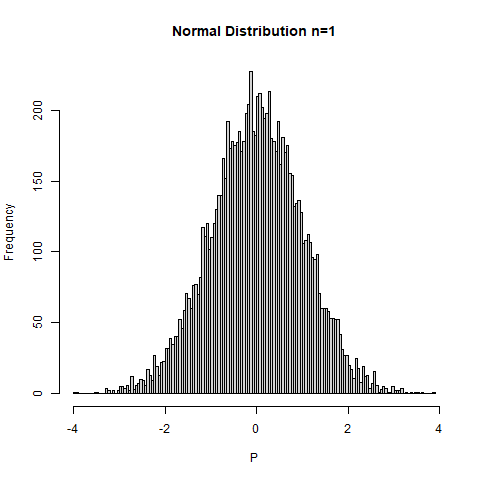
\includegraphics[scale=0.6]{hist1-1.png}
\end{minipage}
\begin{minipage}{0.5\textwidth}
    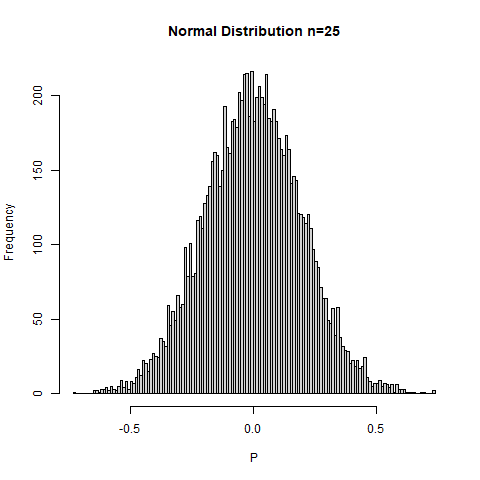
\includegraphics[scale=0.6]{hist1-2.png}
\end{minipage}
\begin{minipage}{0.5\textwidth}
    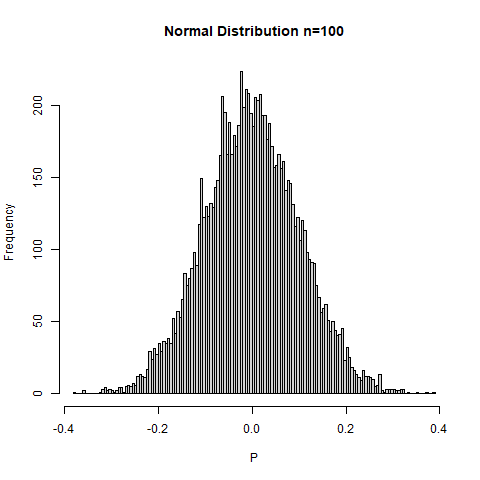
\includegraphics[scale=0.6]{hist1-3.png}
\end{minipage}
\begin{minipage}{0.5\textwidth}
    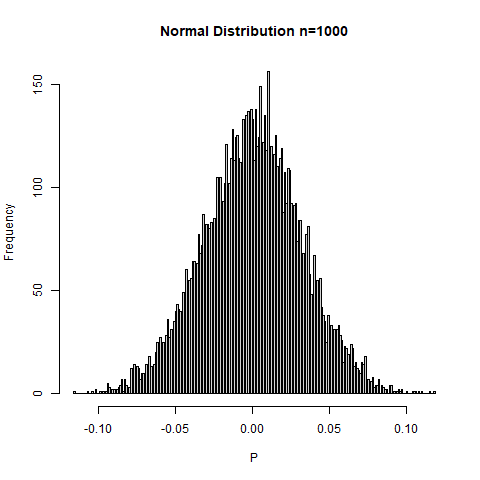
\includegraphics[scale=0.6]{hist1-4.png}
\end{minipage}
\subsection{均匀分布}
\begin{minipage}{0.5\textwidth}
    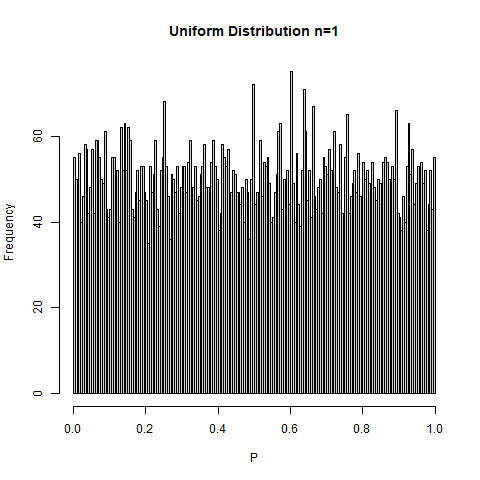
\includegraphics[scale=0.6]{hist2-1.png}
\end{minipage}
\begin{minipage}{0.5\textwidth}
    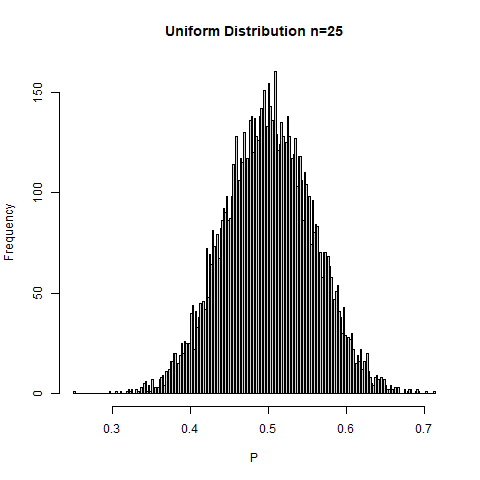
\includegraphics[scale=0.6]{hist2-2.png}
\end{minipage}
\begin{minipage}{0.5\textwidth}
    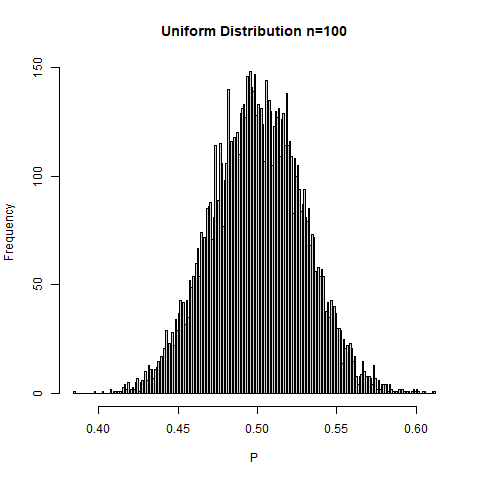
\includegraphics[scale=0.6]{hist2-3.png}
\end{minipage}
\begin{minipage}{0.5\textwidth}
    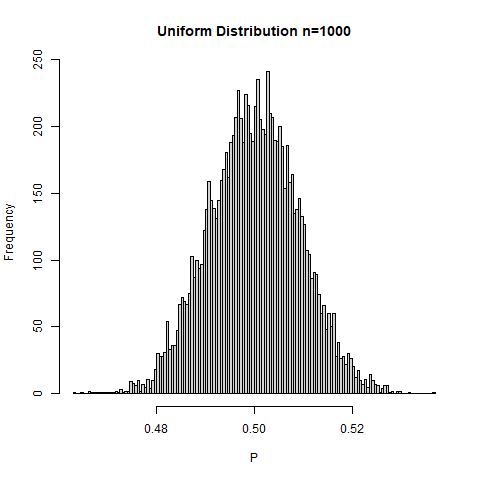
\includegraphics[scale=0.6]{hist2-4.png}
\end{minipage}
\subsection{Cauchy分布}
\begin{minipage}{0.5\textwidth}
    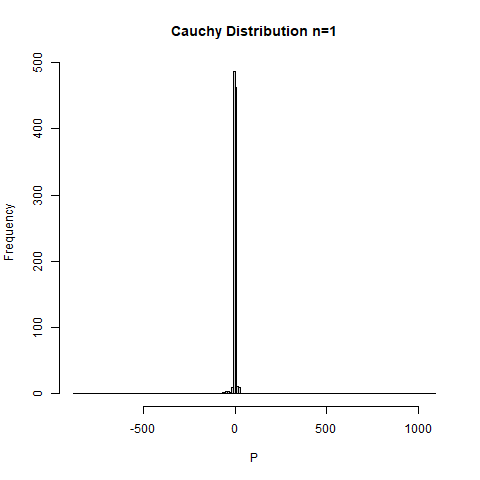
\includegraphics[scale=0.6]{hist3-1.png}
\end{minipage}
\begin{minipage}{0.5\textwidth}
    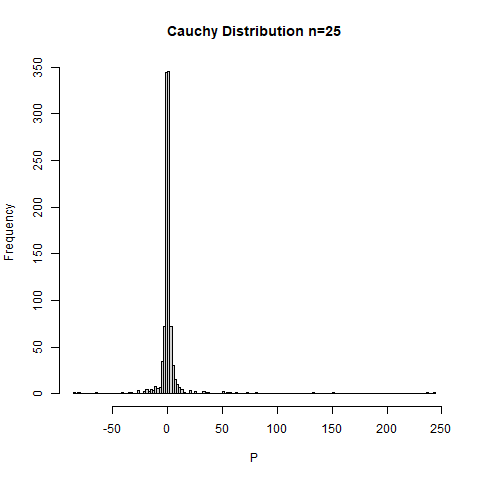
\includegraphics[scale=0.6]{hist3-2.png}
\end{minipage}
\begin{minipage}{0.5\textwidth}
    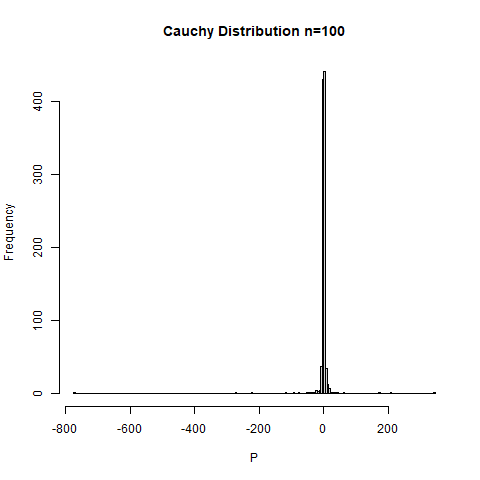
\includegraphics[scale=0.6]{hist3-3.png}
\end{minipage}
\begin{minipage}{0.5\textwidth}
    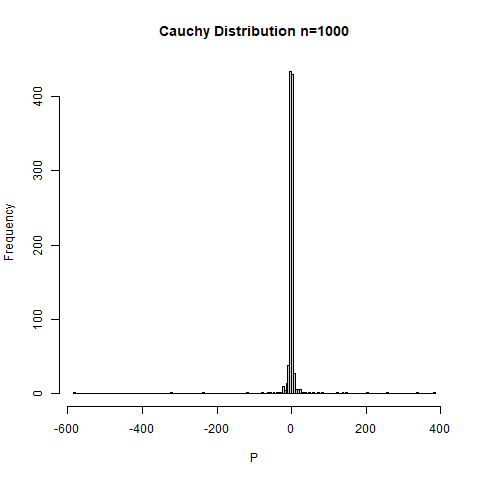
\includegraphics[scale=0.6]{hist3-4.png}
\end{minipage}
\subsection{结论}
正态分布和均匀分布符合中心极限定理,而Cauchy分布不符合,因为Cauchy分布的方差不存在.
\end{CJK}
\end{document}